\chapter{Particle Flow Reconstruction}

One of the goals of this thesis is to build a framework to study the performance of Particl Flow jet performance in Run 2. Therefore this chapter will give an overview of the results that the new algorithm has brought for Run 1.

This chapter starts with an introdution to the Particle Flow algorithm based on the Particle Flow paper \cite{pflow16}. After the description of the steps a brief overview ot the results the algorithm brought for Run 1 are presented. The last section summarizes the updates to the algorithm for Run 2.

\section{The Particle Flow Algorithm}

Recently only either the Calorimeter or the tracker information was used to reconstruct Jets in ATLAS. The Particle Flow algorithm now combines tracker and calorimeter information to achieve better resolution especially at lower energies. The main advantages of including the tracker information into reconstruction are as follows:


\begin{itemize}
\item For low energy charged particles the momentum resolution measured by the tracking detector is superior to the calorimeter.
\item The tracking detector is able to reconstruct soft particles, which would not pass the noise threshold of the calorimeter and therefore not being reconstructed in the calorimeter at all.
\item The ATLAS tracking detector has a superior angular resolution for single charged particles.
\item Low $p_T$ charged particles may be swept out of the cone before reaching the calorimeter by the magnetic field. The tracker information allows to cluster these particles into the jet.
\item The vertex determination possible due to the use of tracks reduces the pileup-contribution considerably.
\end{itemize}

Figure \ref{fig:pflowflowchart} sketches the important steps of the Particle Flow algorithm. The algorithm uses clusters and tracks as input information. The first step is to match a track spatially to a cluster. After a pair has been found the algorithm checks whether the particle's momentum matches the expected energy deposited in the cluster within the expected deviation. Then:
\begin{itemize}
\item If the energy matches the subtraction algorithm starts deciding which calorimeter cells belong to the given jet.
\item If the energy deposited in the cluster is too low the algorithm includes all the clusters in a given area and then starts the subtraction.
\end{itemize}


After the subtraction the algorithm provides not only the modified clusters with the identified remnants but also the tracks and the original unchanged clusters for further analysis.

\begin{figure}[h]
  \centering
  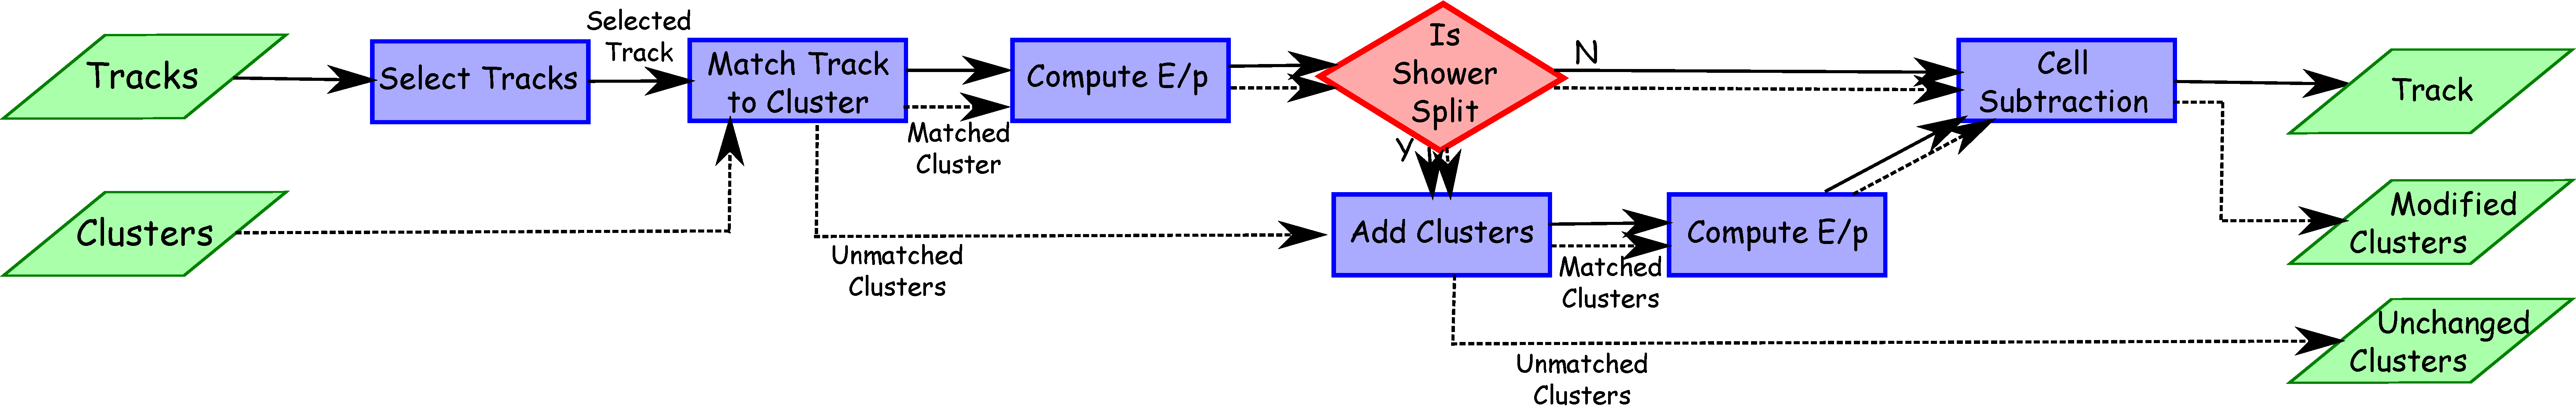
\includegraphics[width=\figwidth]{flowchart.pdf}
  \caption[Flowchart of the steps of the Particle Flow algorithm]{Flowchart of the steps of the Particle Flow algorithm \cite{pflow16}}
  \label{fig:pflowflowchart}
\end{figure}

\subsection{Track selection}

The tracks are selected if they pass certain cuts which are applied n order to minimize the amount of fake tracks. The requirements are at least 9 hits in the PIXEL plus SCT and no missing hits in the PIXEL at all. The tracks have to be in a pseudo-rapidity region of $|\eta|<2.5$ and $\SI{0.5}{\GeV}<p_T<\SI{40}{\GeV}$.

%check with twiki trackselection



\subsection{Clusters}

The calorimeter input informationof the Particle Flow algorithm comes in the form of topological clusters. The construction of these clusters is briefly described here.

The idea of creating topological clusters is to group neighboring cells that exceed the expected noise by a significant amount into collections. 
Each cluster is being constructed around a so called seed cell. A seed cell is a cell for which the deposited energy exceeds the expected noise by four times the standard deviation. If a seed is found all the neighboring cells which exceed the noise by at least two times the standard deviation are added to the cluster. Finally all the cells neighboring these cells are also added to the final cluster.

The final number of cells in a cluster is therefore not static. For more information see the report "Calorimeter Clustering Algorithms: Description and Performance"\cite{cluster08}.


\subsection{Matching track to cluster}

The algorithm tries to match every selected track to one single best-match calorimeter cluster. 
Therefore the distances in $\Delta \phi$ and $\Delta \eta$ from the track extrapolated to the second layer of the EM calorimeter and the topo-clusters have to be calculated. After that the topo-clusters get ranked based on the metric:

\begin{equation}
\Delta R' = \sqrt{\left(\frac{\Delta \phi}{\sigma_{\phi}}\right)^2+\left(\frac{\Delta \eta}{\sigma_{\eta}}\right)^2}
\end{equation}

Where $\sigma_{\eta}$ and $\sigma_{\phi}$ refer to the angular topo-cluster width, computed from the standard deviation of the displacemtens of the topo clusters and $\Delta \phi$ and $\Delta \eta$ are calculated as follows:

\begin{equation}
\Delta \phi = (\phi_{track} - \phi_{cluster})
\Delta \eta = (\eta_{track} - \eta_{cluster})
\end{equation}

If the energy in this cluster is greater than or equal to the energy expected from the track's $p_T$ the algorithm goes to cell subtraction. If the energy in the cluster is smaller than the expected energy all clusters in a cone of $\Delta R < 0.2$ are matched to the track. In that case R is calculated by the metric:

\begin{equation}
\Delta R = \sqrt{(\Delta \phi)^2 + (\Delta \eta)^2}
\end{equation}

If the energy of all the matched clusters still does not match the expected energy the matching failed.

\subsection{Cell Subtraction}

The last step in the Particle Flow algorithm is the cell-wise subtraction of energy deposits to remove noise remnants and determine which energy depositions belong to the matched track or to other neutral objects.
If the energy deposited in the cluster or the set of clusters is lower than the expected energy, the clusters are simply removed. Otherwise, a cell by cell subtraction is performed.

The first step of the cell subtraction is to generate a shower shape from the extrapolated track. Around the extrapolated track direction rings in the $\eta$, $\phi$ plane are generated just wide enough to independently contain at least one cell from the extrapolated position. Furthermore the rings are restricted to one layer and of the same radial size for each layer.
After the generation of rings in each layer the average energy density in each ring is computed and the rings are ranked by energy density in descending order. The layer is not used in any way for this ranking.
The subtraction then starts from the ring with highest energy density and proceeds successively to rings of lower order until the next ring's energy exceeds the remaining expected energy.
If the ring's energy exceeds the energy still to be substracted the energy in each cell is scaled down by the fraction needed to reach the expected energy before the process halts. The remaining cells are removed as remnants if they are consitent within the standard deviation of $\sigma (E/p)$. If the remaining energy is larger than $\sigma (E/p)$ the cells are kept a a neutral Particle Flow object (nPFO).
An example of the process is sketched in figure \ref{fig:sub}. 




\begin{figure}[htbp]
  \centering
  \begin{subfigure}[b]{0.3\figwidth}
    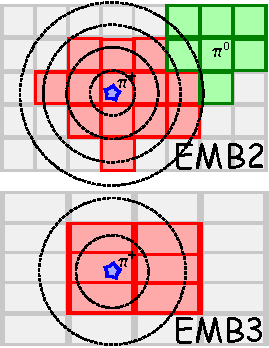
\includegraphics[width=0.25\figwidth]{a}
    \caption{}\label{fig:sub-a}
  \end{subfigure}
  \begin{subfigure}[b]{0.3\figwidth}
    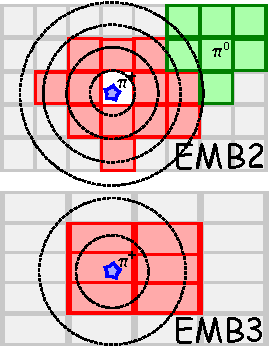
\includegraphics[width=0.25\figwidth]{b}
    \caption{}\label{fig:sub-b}
  \end{subfigure}
  \begin{subfigure}[b]{0.3\figwidth}
    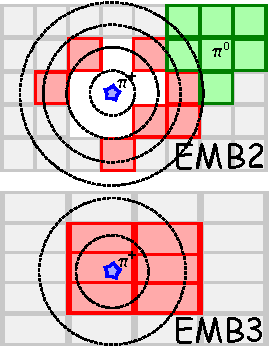
\includegraphics[width=0.25\figwidth]{c}
    \caption{}\label{fig:sub-c}
  \end{subfigure}
  \begin{subfigure}[b]{0.3\figwidth}
    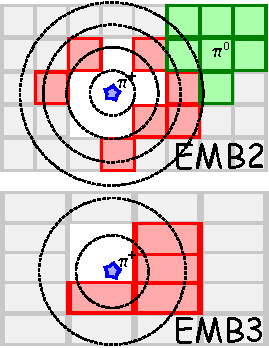
\includegraphics[width=0.25\figwidth]{d}
    \caption{}\label{fig:sub-d}
  \end{subfigure}
    
    
  \begin{subfigure}[b]{0.3\figwidth}
        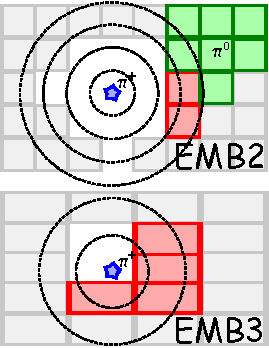
\includegraphics[width=0.25\figwidth]{e}
        \caption{}\label{fig:sub-e}
  \end{subfigure}
  \begin{subfigure}[b]{0.3\figwidth}
        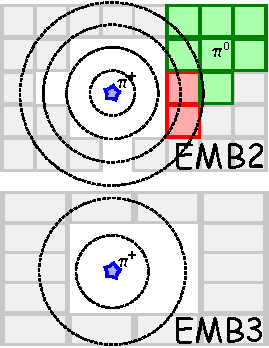
\includegraphics[width=0.25\figwidth]{f}
        \caption{}\label{fig:sub-f}
  \end{subfigure}
  \caption{Example of cell subtraction. In red the energy deposited by the $\pi ^+$ of interest are shown and in green a cluster from a $\pi ^0$ is shown. The algorithm succesfully determines the cells belonging to the $\pi ^+$ and removes them while leaving the green cells as remnants. Only in subfigure \ref{fig:sub-f} part of the green cells is removed while part of the red cells remain because both fall into the same subtraction ring. \cite{pflow16}}
  \label{fig:sub}
\end{figure}

%add a reference here. wildcard there

\subsection{Eflow Rec performance studies}

The results extracted from the Particle Flow paper \cite{pflow16} show the impact of the algorithm on the angular resolution and on the rejection of pileup jets. This section briefly summarizes the improvements in the Particle Flow jet performance compared with other jet collections based on calorimeter information (LC). Figure \ref{fig:etarun1} and \ref{fig:phirun1} show the improvements in angular resolution while figure \ref{fig:pileuprun1} displays the increased rejection of fake jets for the new algorithm. LC+JES jets are the jets using the old algorithm and JVF in figure \ref{fig:pileuprun1} refers to the Jet Vertex Fraction representing the amount of energy in the jet originating from the original vertex.

The plots clearly demonstrate that the Particle Flow algorithm does improve the angular resolution in low $p_T$ regions while having no drawback for higher $p_T$ regions. The pileup contribution is also mediated massively even in comparison to the usage of a cut on the JVT. The region of effect is restricted to $|\eta|<\num{2.5}$ because only this region of pseudorapidity is covered by the Inner Detector. Only the momentum resolution shown in figure \ref{fig:ptrun1} worsens using the old reconstruction for high $p_T$ regions.
%JVT sentence


\begin{figure}[h]
  \centering
  \begin{subfigure}[b]{0.5\figwidth}
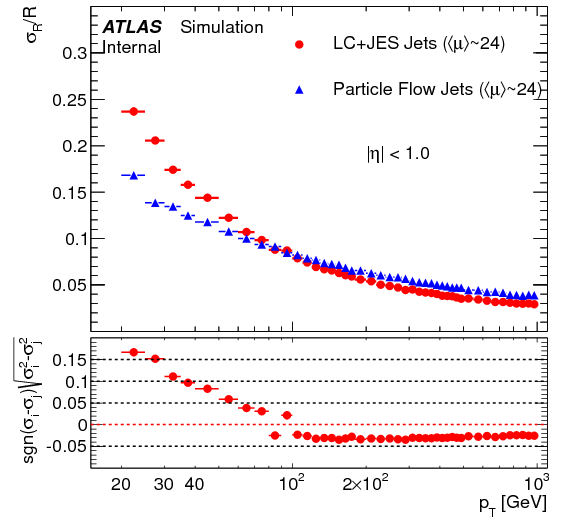
\includegraphics[width=0.5\figwidth]{ptrun1.png}
\caption[Momentum resolution of Particle Flow]{Momentum resolution of Particle Flow jets \cite{pflow16}}
\label{fig:ptrun1}
\end{subfigure}
\quad
  \begin{subfigure}[b]{0.5\figwidth}
  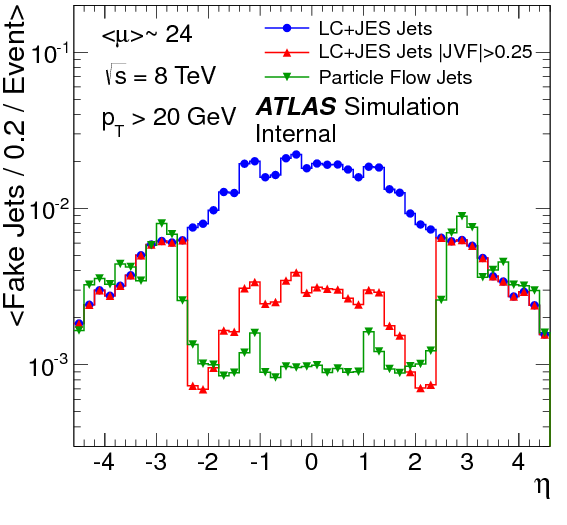
\includegraphics[width=0.5\figwidth]{pileuprun1.png}
  \caption[Pileup comparison of EM-Topo Jets and Particle Flow jets]{Pileup comparison of EM-Topo Jets and Particle Flow jets \cite{pflow16}}
  \label{fig:pileuprun1}
  \end{subfigure}
\end{figure}



\begin{figure}[h]
  \centering
  \begin{subfigure}[b]{0.5\figwidth}
  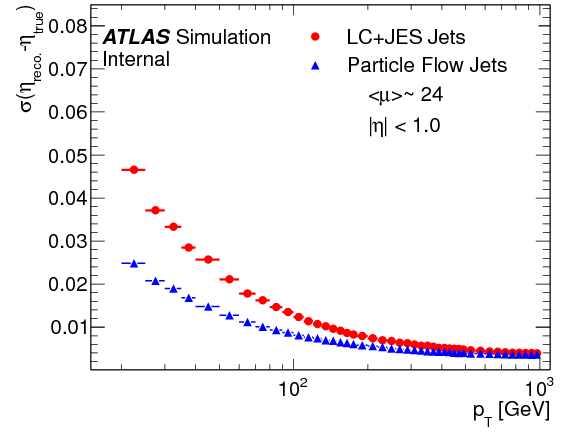
\includegraphics[width=0.5\figwidth]{etarun1.png}
  \caption[Improvements in $\eta$ resolution for Particle Flow Jets]{Improvements in $\eta$ resolution for Particle Flow Jets \cite{pflow16}}
  \label{fig:etarun1}
  \end{subfigure}
  \quad
  \begin{subfigure}[b]{0.5\figwidth}
  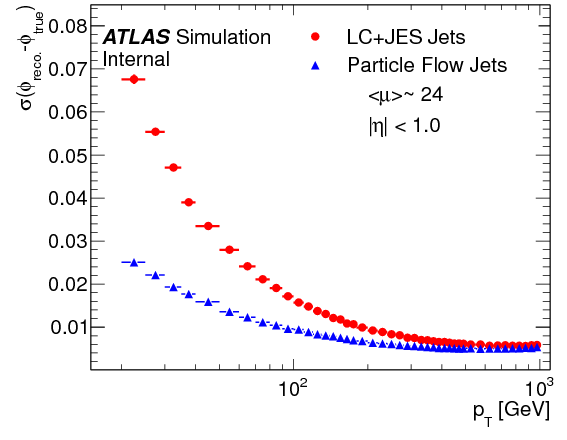
\includegraphics[width=0.5\figwidth]{phirun1.png}
  \caption[Improvements in $\phi$ resolution for Particle Flow Jets]{Improvements in $\phi$ resolution for Particle Flow Jets \cite{pflow16}}
  \label{fig:phirun1}
  \end{subfigure}
\end{figure}





\subsection{Recent updates in eflowrec}

The description of the Particle Flow algorithm given in this thesis is based on the algorithm implemented in Run 1.

Recently some changes have been included and they are briefly mentioned in this section:

\begin{itemize}
\item The track selection has been updated to the tight track criteria of the ATLAS tracking group.
\item In dense environments where the association of energy deposited in the calorimeter to the track can not be done properly th subtraction is not applied.

\end{itemize}


%Here I want to explain what tools are used for PFlow already and what tools are %missing.
%Then I should focus on which tools have been implicitly upgraded
%Problematic right now are the cleaning the trigger matching the pileup reweithing %and the complete JES